% Created 2021-10-07 Thu 15:58
% Intended LaTeX compiler: pdflatex
\documentclass[presentation,aspectratio=169, usenames, dvipsnames]{beamer}
\usepackage[utf8]{inputenc}
\usepackage[T1]{fontenc}
\usepackage{graphicx}
\usepackage{grffile}
\usepackage{longtable}
\usepackage{wrapfig}
\usepackage{rotating}
\usepackage[normalem]{ulem}
\usepackage{amsmath}
\usepackage{textcomp}
\usepackage{amssymb}
\usepackage{capt-of}
\usepackage{hyperref}
\usepackage{khpreamble}
\usepackage{amssymb}
\usepgfplotslibrary{groupplots}
\newcommand*{\shift}{\operatorname{q}}
\definecolor{ppc}{rgb}{0.1,0.1,0.6}
\definecolor{iic}{rgb}{0.6,0.1,0.1}
\definecolor{ddc}{rgb}{0.1,0.6,0.1}
\def\ucolor{blue!80!black}
\def\ycolor{green!60!black}
\newcommand*{\incolor}[1]{\textcolor{\ucolor}{#1}}
\newcommand*{\outcolor}[1]{\textcolor{\ycolor}{#1}}
\usetheme{default}
\author{Kjartan Halvorsen}
\date{\today}
\title{Anti-windup}
\hypersetup{
 pdfauthor={Kjartan Halvorsen},
 pdftitle={Anti-windup},
 pdfkeywords={},
 pdfsubject={},
 pdfcreator={Emacs 26.3 (Org mode 9.4.6)}, 
 pdflang={English}}
\begin{document}

\maketitle

\section{PID tuning - (Smith and Corripio) Ziegler Nichols}
\label{sec:orgf8a8844}
\begin{frame}[label={sec:orge8e09d0}]{The PID - practical form}
\definecolor{ppc}{rgb}{0.1,0.1,0.6}
\definecolor{iic}{rgb}{0.6,0.1,0.1}
\definecolor{ddc}{rgb}{0.1,0.5,0.1}

\begin{center}
  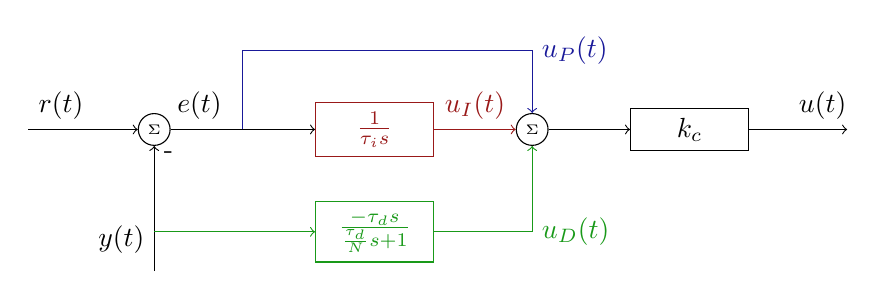
\begin{tikzpicture}[node distance=22mm, block/.style={rectangle, draw, minimum width=15mm}, sumnode/.style={circle, draw, inner sep=2pt}]

    \node[coordinate] (input) {};
    \node[sumnode, right of=input, node distance=16mm] (sum) {\tiny $\Sigma$};
    \node[color=iic,block, right of=sum, node distance=28mm] (ii)  {$\frac{1}{\tau_is}$};
    \node[color=ppc, coordinate, above of=ii, node distance=10mm] (pp)  {};
    \node[color=ddc,block, below of=ii, node distance=13mm] (dd)  {$\frac{-\tau_ds}{\frac{\tau_d}{N}s + 1}$};
    \node[sumnode, right of=ii, node distance=20mm] (sum2) {\tiny $\Sigma$};
    \node[block, right of=sum2, node distance=20mm] (gain)  {$k_c$};
    \node[coordinate, below of=sum, node distance=18mm] (feedback) {};
    \node[coordinate, right of=gain, node distance=20mm] (output) {};

    \draw[->] (input) -- node[above, pos=0.3] {$r(t)$} (sum);
    \draw[->] (sum) -- node[above, pos=0.2] {$e(t)$} node[coordinate] (mm) {}  (ii);
    \draw[->] (gain) -- node[above, near end] {$u(t)$} (output);
    \draw[->] (feedback) -- node[left, near start] {$y(t)$} node[right, pos=0.95] {-} (sum);
    \draw[->, color=ppc] (mm) |- (pp) -| node[right,] {$u_P(t)$} (sum2);
    \draw[->, color=ddc] (feedback |- dd) -- node[above, pos=0.95] {} (dd);
    \draw[->, color=ddc] (dd) -| node[right,] {$u_D(t)$} (sum2)  ;
    \draw[->, color=iic] (ii)  -- node[above,] {$u_I(t)$} (sum2);
    \draw[->] (sum2) -- node[above, near end] {} (gain);

  \end{tikzpicture}
\end{center}
\end{frame}

\section{Windup}
\label{sec:org9d89f2b}

\begin{frame}[label={sec:orgfa6a877}]{Integral windup}
\href{https://tecdemonterrey.instructuremedia.com/embed/6fb197b1-38a6-4938-b622-b25d4a45efcc}{Video by Tomás Alejandro Lugo Salinas (MTY)} 
\end{frame}

\section{Anti-windup}
\label{sec:org2f751ae}


\begin{frame}[label={sec:org4a22b68}]{Anti-windup using back-calculation}
   \begin{center}
 	  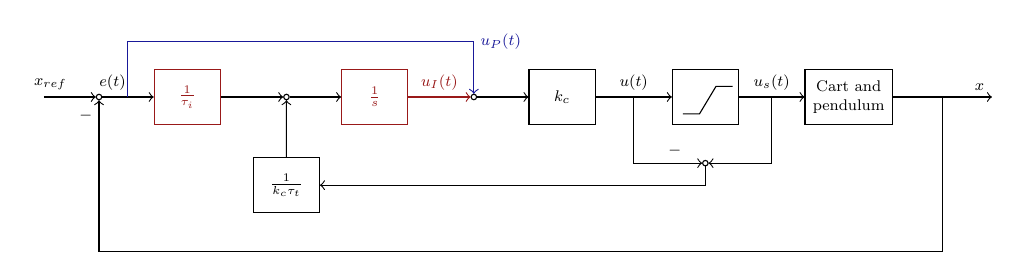
\begin{tikzpicture}[every node/.append style={transform shape}, scale = 0.7, font=\footnotesize,
	block/.style={rectangle, draw, minimum width=12mm, minimum height=10mm, inner sep=4pt},
	amp/.style = {regular polygon, regular polygon sides=3,
              draw, fill=white, text width=1em,
              inner sep=1pt, outer sep=0mm,
              shape border rotate=-90},
	      summ/.style = {circle, draw, inner sep = 1pt},]
	 \node[block, align=center] (motor) at (0,0) {Cart and \\pendulum};
	 \node[coordinate, right of=motor, node distance = 26mm,] (output) {};
	 \node[block, left of=motor, node distance=26mm] (saturation) {};

	 \node[block, left of=saturation, node distance=26mm] (gain)  {$k_{c}$};
	 
	 \node[summ, left of=gain, node distance=16mm] (sum2) {};
	 \node[color=iic,block, left of=sum2, node distance=18mm] (int)  {$\frac{1}{s}$};
	 \node[summ, left of=int, node distance=16mm] (sumint) {};
	 \node[color=iic,block, left of=sumint, node distance=18mm] (ii)  {$\frac{1}{\tau_{i}}$};
	 \node[color=ppc, coordinate, above of=ii, node distance=10mm] (pp)  {};
	 \node[summ, left of=ii, node distance=16mm] (sumsp) {};
	 \node[coordinate, left of=sumsp, node distance = 10mm,] (setpoint) {};

       \draw[->] (sumsp) -- node[above, pos=0.2] {$e(t)$} node[coordinate] (mm) {}  (ii);
       \draw[->] (gain) -- node[coordinate] (idmeas) {} node[above, ] {$u(t)$} (saturation);
       \draw[->, color=ppc] (mm) |- (pp) -| node[right,] {$u_P(t)$} (sum2);
       \draw[->, color=iic] (int)  -- node[above,] {$u_I(t)$} (sum2);
       \draw[->] (sum2) -- node[above, near end] {} (gain);



	 \draw[->] (setpoint) -- node[above, very near start ] {$x_{ref}$} (sumsp);
	 \draw[->] (saturation) -- node[coordinate, ] (satmeas) {} node[above,] {$u_s(t)$} (motor);
	 \draw[->] (motor) -- node[coordinate] (meas) {} node[above, very near end] {$x$} (output);
	 \draw[->] (meas) -- node[right] {} ++(0,-28mm) -| node[pos=0.95, left] {$-$} (sumsp);

	 % Anti-windup
	 \draw ($ (saturation.south west) + (2mm, 2mm) $) -- ++(3mm, 0) -- ++(3mm, 5mm) -- ++(3mm, 0);
	 \node[block, below of=sumint, node distance=16mm] (back) {$\frac{1}{k_{c}\tau_t}$};
	 \node[summ, below of=saturation, node distance=12mm] (sumsat) {};
	 \draw[->] (satmeas) |- node[above, pos=0.8] {} (sumsat);
	 \draw[->] (idmeas) |- node[above, pos=0.8] {$-$} (sumsat);
	 \draw[->] (sumsat) |- (back);
	 \draw[->] (back) -- (sumint);
	 \draw[->] (ii) -- (sumint);
	 \draw[->] (sumint) -- (int);
	 

	 \node[coordinate, right of=back, node distance=2cm] (sat) {};
  
\end{tikzpicture}
\end{center}

\alert{Activity} Assume \(e(t)=0\) and determine the transfer function from \(u_s(t)\) to \(u(t)\).
\end{frame}
\end{document}